\NewsTitle{Intelligent Machine Condition Monitoring for Cyber-Physical Systems}
\NewsAuthor{Arkadeb Ghosal, Kaushik Ravindran, Patricia Derler, Hugo A. Andrade, and Jeannie Falcon\\%alphabetical order?
National Instruments Corporation}

% Titles:

%Cybernetics for Intelligent Machine Condition Monitoring\\and Control Applications (first choice)\\ 
% Cybernetics for intelligent monitoring
% Cybernetics for intelligent machine monitoring
% Cybernetics for intelligent machine condition monitoring

% Notes about content:

% Trend on large scale distributed sensor machine monitors
% Requires: 
% 1. monitoring the condition of indivudual parts
% 2. transmiting data and calculating the condition indicators
% 3. managing deployment of large sensor nodes

% Making data available for remote viewing and analysis

% NI InsightCM is such is an enterprise level solution to such a problem/requirement

% Modern day IIoT has enabled large distributed systems with over 30,000 sensors and 10,000 nodes. 
% Given the scale we need introduce automatic monitoring, that is node and application specific.
% In the case of rotating machinery, we have large body of knowledge on analytics. 

% Cybernetics include libraries that collect "big data" across the many nodes, and the run
% analtics for indivudals nodes, acrross region and acrross full deploymnenbts. 


% \input{doc/Intro}
\section{Introduction} 

%http://www.ni.com/internet-of-things/ 
%By 2020, more than 50 billion devices will be digitally connected, representing $19 trillion in business opportunity (original statement by Cisco)
% Adny Chang's article in http://issuu.com/xcelljournal/docs/xcell_journal_issue_92
% According to Gartner Inc., an estimated 4.9 billion connected devices will be used in 2015, rising to 25 billion in 2020

Modern day Industrial Internet of Things (IIoT) applications are large heterogeneous distributed systems with over 30,000 sensors and 10,000 nodes.
Trends indicate a tremendous growth in the number of connected components over the coming years.
Gartner Research predicts over 20~billion interconnected devices by 2020, representing a \$3 trillion business and technology opportunity \cite{Gartner_IoT_2020}.
%Predictions for the number of interconnected devices by 2020 range from 25 billion (Gartner Inc.) to 50 billion (Cisco), representing a \$19 trillion dollar business and technology opportunity.
Lee et al. refer to this emerging global cyber-physical network as the \emph{TerraSwarm}, encompassing trillions of sensors and actuators deployed across the planet \cite{SwarmAtEdgeOfCloud}.
These applications will dynamically assemble sensors and computation nodes, aggregate and process large quantities of data, and transfer decisions to actuators and controllers, while meeting tight performance requirements and cost constraints.

Cyber-physical networked systems can generate gigabytes and potentially terabytes of sensor data about the condition and operation of the system.
For example, the condition monitoring solution for the Victoria Line of the London Underground rail system yields 32 TB of data every day \cite{NITrendWatch2016}. 
In the midst of this explosion of engineering and measurement data, it has become imperative for systems to incorporate a sound management strategy to aggregate the data, conduct diagnostic analytics about the condition of the system, and facilitate predictive maintenance to reduce downtimes and maximize efficiency.
%Monitoring solutions must provide efficient analytics at the edges of the system and smart enterprise management to derive insight into patterns and trends in the operation of the system.
Given the cost and complexity of modern cyber-physical systems, it is important that the monitoring solution be scalable and customizable to meet changing application requirements.

Nevertheless, with the advances in sensing and networking technologies, adding measurements to systems has become easier and cost-effective. 
Intelligence of data acquisition devices and sensors has drastically increased and become more decentralized, with processing elements moving closer to the sensor.
In addition to measurement devices getting smarter, smart sensors have emerged that integrate sensing, signal conditioning, embedded processing, and digital interfacing into the sensor node itself. 

As processing moves closer to the sensor, innovation in measurement system software is required to efficiently push analytics to the edge. 
Future software for edge-based systems will be able to quickly configure and manage thousands of networked measurement devices and push a myriad of analytics and signal processing to those nodes. 
Going forward, systems must transition to smarter, software-based measurement nodes to keep up with the amount of analog data and derive insights about patterns and trends in the operation of the system.
The ``smart edge'' needs specialized software and platform solutions to perform local control and data acquisition and interconnect with entire networks of intelligent ``systems of systems'' \cite{NITrendWatch2016}.

In this paper, we discuss advances in intelligent machine condition monitoring for cyber-physical networked systems and recent technologies in this area. 
Section 2 of this paper reviews key components and techniques in a machine condition monitoring solution. 
Section 3 then presents an industrial tool called InsightCM from National Instruments and discusses an application case study.

%Major players in the marketplace include Br\"{u}el \& Kjaer Vibro, ClampOn AS, Corrpro Companies Inc., Data Physics Corporation, DLI Engineering Corp, Emerson Process Management, FLIR Systems Inc., GE Energy, Honeywell Process Solutions, ITT Corporation, Kittiwake Developments Limited, PCB Piezotronics Inc., Rockwell Automation Inc., Rohrback Cosasco Systems, Scientific Monitoring Inc., Shinkawa Electric Co., Ltd., SKF Condition Monitoring Inc., SPM Instrument AB, The Timken Company, among others \cite{ResarchandMarkets15}.

%EETimes: http://www.eetimes.com/document.asp?doc_id=1320763 
%“sensors are everywhere and in every form”

%ehttp://www.reliableplant.com/Read/28292/Global-machine-condition-monitoring
%Condition monitoring has gained importance as companies critically focused on asset utilization and productivity.
%The need for eliminating catastrophic downtimes due to unexpected breakdowns and unnecessary maintenance costs will continue to drive the adoption of condition monitoring solutions across several industries.

%Discuss:
%Title
%No NI refs in sec 2.
%More refs.
%Summary?
%Expand scope to cybernetics or keep current scope to MCM for CPS
%Move major players to sec 3
%Move MCM disc to sec 2
% Somewthing about crio
%Something about duke energy analysis

%One of the few industries to flourish in adversity is the machine condition monitoring equipment market. A traditionally resilient vector of the industrial equipment market, machine condition monitoring equipment has recorded hardy growth against a backdrop of increased focus on reducing plant operating costs by reducing maintenance costs, optimizing maintenance activities during planned shutdowns and lowering the instances of unscheduled outages. 

%

%http://www.researchandmarkets.com/reports/3493625/machine-condition-monitoring-market-by-monitoring

%Brüel \& Kjær Vibro, ClampOn AS, Corrpro Companies Inc., Data Physics Corporation, DLI Engineering Corp, Emerson Process Management, FLIR Systems Inc., GE Energy, Honeywell Process Solutions, are some major players in the market. 

%Outline: Generic trends in cybernetics. Motivate need for monitoring lots of data. MCM becomes important for cybernetics. List companies in MCM. 

%Xilinx Xcell 92: http://www.xilinx.com/publications/archives/xcell/Xcell92.pdf

%“Mac hine Condition Monitoring Equipment: A Global Strategic Business Report” announced by Global Industry Analysts Inc., 
%http://www.strategyr.com/Marketresearch/Machine_Condition_Monitoring_Equipment_Market_Trends.asp
\section{Machine Condition Monitoring}
% \section{Machine Condition Monitoring And Control}

Machine condition monitoring (MCM) is the process of monitoring the condition of a machine with the intent to predict mechanical wear and failure. Vibration, noise, and temperature measurements are often used as key indicators of the state of the machine. 
Trends in the data provide health information about the machine and help detect machine faults early, which prevents unexpected failure and costly repair \cite{MCMHandbook}. % I would not cite NI here but, if necessary, find a more general reference. NI did not invent MCM ;) \cite{MCM_NI}
%Machine condition monitoring solutions enable predictive maintenance to reduce machine repairs to maximize efficiency.
The need to eliminate catastrophic downtimes due to unexpected breakdowns and unnecessary maintenance costs has made condition monitoring critical for asset utilization and productivity across diverse industries.
The global machine condition monitoring equipment market is expected to grow at a CAGR of 7.6\% between 2015 and 2020 from \$1.5 billion in 2014 to \$2.5 billion by 2020 \cite{ResarchandMarkets15}.

MCM provides vital information about the health of a machine. An organization can use this information to detect warning signs early and avoid unscheduled outages, optimize machine performance, and reduce repair time and maintenance costs. Figure~\ref{fig:MCM_Timeline}  shows a typical machine failure example and the warning signs. The user can detect failure signs months before repair is required, allowing for proper maintenance scheduling and shutdown.

\begin{figure}[ht!]
    \centering
    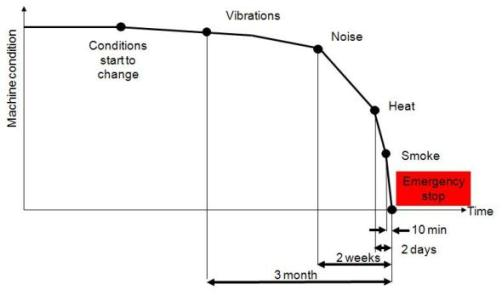
\includegraphics[width=.50\textwidth]{MCM_Timeline}
    \caption{The warning signs of machine failure}
    \label{fig:MCM_Timeline}
\end{figure}

As shown in Figure~\ref{fig:MCM_Timeline}, vibrations are the first warning sign that a machine is prone to failure. This warning sign can provide up to three months of lead time before the actual failure date. Monitoring this data with vibration analysis hardware and software helps predict this failure early and schedule proper maintenance \cite{Randall_VibrationbasedCM}. 

% \subsection{Types of Machine Condition Monitoring}

% Each of the five main varieties of machine condition monitoring serves a different role.
% \begin{itemize}
% \item \emph{Route-based monitoring} involves a technician recording data intermittently with a handheld instrument. This data is then used for trending to determine if more advanced analysis is needed.
% \item \emph{Portable machine diagnostics} is the process of using portable equipment to monitor the health of machinery. Sensors are typically permanently attached to a machine and portable data acquisition equipment is used to read the data.
% \item \emph{Factory assurance test} is used to verify that a finished product meets its design specifications and to determine possible failure modes of the device. 
% \item \emph{Online machine monitoring} is the process of monitoring equipment as it runs. Data is acquired by an embedded device and transmitted to a main server for data analysis and maintenance scheduling. 
% \item \emph{Online machine protection} is the process of actively monitoring equipment as it runs. Data is acquired and analyzed by an embedded device. Limit settings can then be used to control turning on and off machinery.
% \end{itemize}

There are five main types of machine condition monitoring.
\emph{Route-based monitoring} involves a technician recording data intermittently with a handheld instrument. This data is then used to determine if more advanced analysis is needed.
\emph{Portable machine diagnostics} is the process of using portable equipment to monitor the health of machinery. Sensors are typically permanently attached to a machine and portable data acquisition equipment is used to read the data.
\emph{Factory assurance test} is used to verify that a finished product meets its design specifications and to determine possible failure modes of the device. 
\emph{Online machine monitoring} is the process of monitoring equipment as it runs. Data is acquired by an embedded device and transmitted to a main server for data analysis and maintenance scheduling. 
\emph{Online machine protection} is the process of actively monitoring equipment as it runs. Data is acquired and analyzed by an embedded device. Limit settings can then be used to control turning on and off machinery.

% \subsection{Sensors and Signal Processing}

Direct machine condition monitoring is accomplished via sensors, of which the most prevalent types are: accelerometers, tachometers, and proximity probes.  

\begin{itemize}

\item \emph{Accelerometers} are used to monitor vibrations of a machine. These are transducers for measuring the dynamic acceleration of a physical device, and are important to machine monitoring because they monitor system vibrations, which can be used to predict the life cycles of parts and to detect faults in machinery. Among the most common transducers are piezoelectric accelerometers, unbonded strain gage accelerometers, vibrating element accelerometers, and Hall effect accelerometers.

\item \emph{Tachometers} are used to determine the rotational speed of a shaft to provide phase information for the vibration data. These are transducers for measuring the rotational speed of a physical device, and are important to machine monitoring because they provide rotational speed as well as phase information, so that frequency components can be matched to shaft speed and position. Drag torque tachometers are among the most common. 

\item \emph{Proximity Probes} are used to monitor the movement of a shaft. These are transducers for measuring the displacement of a physical device, and are important to machine monitoring because they monitor the movement of a rotating shaft. Proximity probes are usually found in 90-degree offset pairs to map an X-Y plot of the shaft movement. Then imperfections such as misalignment of the shaft, faulty bearings, or other external factors preventing perfect rotation can be prevented. 

\end{itemize}

Most machine condition monitoring sensors require some form of signal conditioning to optimally function, such as excitation power to an accelerometer. Filtering on the signal is also common, to reduce both line noise and unwanted frequency ranges. Once the signals have been acquired, software-based signal processing is used to analyze and display the data from rotating machinery. The analysis can include calculation of overall vibration level (RMS, peak, crest factor); integration from acceleration to velocity or displacement; operation of  online order analysis such as order tracking, order extraction, and order spectra computation; processing of digital and analog tachometer signals; application of limit testing on time data or power spectra; and drawing of a variety of plots ranging from spectral maps to time based plots.

%spectral maps, color maps, waterfall plots, cascade plots, Bode plots, polar plots, orbit plots, time base plots, shaft centerline plots, and Campbell (intensity) plots.

% \subsection{Application Areas}
% Condition monitoring is used in a wide variety of industries. The following is a brief overview of how it works in just a few of them. Certainly condition monitoring can play an important role in any machine with vibrations.

% \subsubsection{Wind Energy}

% To be competitive in the energy market, wind turbines must be operated as cheaply as possible. Maintenance costs for their often remote locations are typically quite high, so route-based monitoring or portable diagnostics systems often don't make sense.  

% Online machine monitoring is often used to monitor wind turbines online from a central location. Technicians can then be deployed to the remote wind farm locations only when maintenance is actually needed.

% Additionally, as companies design larger and more efficient direct-drive turbines, the need for more advanced factory assurance tests becomes increasingly important. Large test cells will need to be built that can monitor turbine designs for up to weeks at a time to verify new multimegawatt designs.

% \subsubsection{Oil and Gas}

% As the cost of reaching oil and gas reserves increases, reducing the operating and maintenance costs of oil and gas assets grows increasingly important. Pumps and drills are often in remote locations where technician expenses are high.

% Using online condition monitoring techniques, you can monitor pumps, wells, and refineries from a central location and only deploy maintenance personnel when necessary, saving operating and maintenance costs.

% The oil and gas industry is also increasingly under pressure for improved safety and oversight. Condition monitoring offers the opportunity to discover possible defects weeks before a technician may find them, and it provides advantages over performing maintenance at only manufacturer-recommended intervals, which may not be early enough to prevent a catastrophic failure.






%\section{NI InsightCM Enterprise for Condition Monitoring}
\section{Condition Monitoring Tools}

There are many commercial tool offerings for machine condition monitoring.
Major players in the marketplace include Br\"{u}el \& Kj{\ae}r Vibro, ClampOn AS, Data Physics Corporation, DLI Engineering Corp, Emerson Process Management, FLIR Systems Inc., GE Energy, Honeywell Process Solutions, among others \cite{ResarchandMarkets15}. 
We now introduce one such MCM tool; 
National Instruments' (NI) InsightCM\textsuperscript{TM} Enterprise~\cite{InsightCMBrochure15}. 
InsightCM is an online MCM tool for monitoring 
%acquires and analyzes sensory information, generates alarms, allows maintenance specialists to %visualize and manage data, and simplifies deployment of large numbers of monitoring systems. It 
health of critical rotating machinery and auxiliary rotating equipment. The goal is to optimize machine performance, maximize up-time, reduce maintenance costs, and increase safety.
This solution allows maintenance specialists to
acquire, analyze, visualize, and manage sensor data throughout the life cycle to draw diagnostic conclusions, manage alarms based on calculated features and sensor measurements,
remotely configure, monitor, and manage acquisition devices, as well as
authenticate users and devices to address network security concerns. By integrating into the IT infrastructure the tool can interact with existing databases and enterprise software. 

Figure~\ref{fig:insightcm-architecture} illustrates key components of the InsightCM solution: monitoring systems, server for data management and analysis, data explorer clients, and management infrastructure.

\begin{figure}[ht]
    \centering
    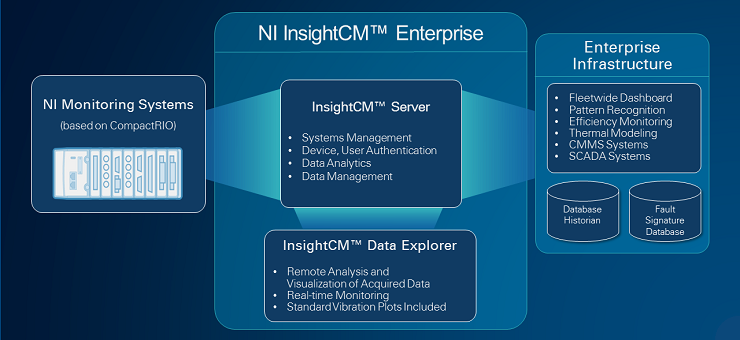
\includegraphics[width=.8\textwidth]{InsightCM_Architecture}
    \caption{NI Insight\textsuperscript{TM} Architecture}
    \label{fig:insightcm-architecture}
\end{figure}

%With the InsightCM Enterprise solution (Figure~\ref{fig:insightcm-architecture}), data is automatically acquired using CompactRIO-based NI Condition Monitoring Systems, and transmitted to the server where it is stored \cite{ni_crio}. 
%The NI InsightCM Server software calculates condition indicators and manages the CompactRIO systems. 
%The data is then avaialable for remote viewing and analysis using the NI InsightCM Data Explorer client application. 
%Data is also exportable as tags to third-party software packages running at the enterprise IT level.

%NI InsightCM\textsuperscript{TM} Enterprise solution consists of four main components (Figure~\ref{fig:insightcm-architecture}): \emph{CompactRIO-based NI Condition Monitoring Systems}, \emph{InsightCM\textsuperscript{TM} Data Explorer}, \emph{InsightCM\textsuperscript{TM} Server} and interface with existing enterprise architecture.


The monitoring devices at the edges of the system are NI CompactRIO platforms \cite{ni_crio}.
These devices, in addition to sensors and I/O modules, have processing and reconfigurable components for inline data processing, control analytics, network communication, and timing.
The CompactRIO devices supports a range of analog and digital sensors, such as proximity probes, accelerometers, pressure sensors, voltage and current sensors, thermocouples, and temperatur detectors. 
%Data is automatically acquired and transmitted to the server where it is stored. 
The monitoring system supports periodic monitoring as well as observation of important transient events such as start-ups and coast-downs. 
The {\em periodic recorder mode} allows data logging based on configurable time intervals, measurements, and user triggers. 
Dynamic waveform and static measurement sensors account for 80\% of measurements in a predictive maintenance program, suitable for replacing traditional, manual diagnostic rounds. 
The {\em transient recorder mode} streams time waveform data during transient events at run-up and coast-down until steady state is maintained, and includes support for accelerometers, velocity meters, and proximity probes. 

%NI InsightCM\textsuperscript{TM} S
The server delivers 
%in-motion -- what is in-motion analytics?
analytics coupled with management of CompactRIO systems, data, and alarms. The server software manages reliable, loss-less communication across the entire architecture and includes capabilities to configure, view, and manage the remote acquisition systems. 
The software processes dynamic waveform data and analyzes RMS, peak-peak, true-peak, derived-peak, DC gap, crest factor, and spectral bands. It also supports custom measurements like bearing, gear, and other fault frequencies. Additionally, the server provides a security layer to authenticate and protect sensor and server data.

%NI InsightCM\textsuperscript{TM} Data Explorer provides 
The data explorer provides
%in-depth, -- sounds like a marketing term - unnecessary?
interactive visualization and analysis of real-time and historical offline data stored in the server. The software package helps in remotely analyzing raw time-series data and results, drawing comparisons and viewing historical trends with support for standard vibration plots. The data explorer provides two modes: one for viewing periodically acquired data and one for viewing previously captured transient events. Users can detect imbalances, bent shafts, misalignment, bearing defects, and other faults in rotating machinery, and determine actions that need to be taken as part of diagnosis and maintenance procedures.

InsightCM has been widely used across multiple industrial domains including traditional power generation, oil and gas, renewable power generation, transportation and aerospace, heavy equipment, and manufacturing~\cite{MCM_UC_NI}. We discuss the use of InsightCM for a power grid monitoring application.

Duke Energy \cite{dukewebsite} is the largest power generation holding company in the US with a diversified energy portfolio mix and the capability to generate 58GW across 80 plants. Data used to be collected manually in periodic rounds on assets such as turbines, transformers, boilers, radiators, valves, motors, pumps, fans, and generators. The typical measurements include motor current, lube oil level, vibration, pressure, performance, and thermography. In this approach, 80\% of the effort was spent on data collection, and 20\% on analytics. Besides being labor intensive (about 60000 rounds/month), this approach has limited instrumentation and inconsistent diagnostics, which severely constrains the analysis.
By employing InsightCM for condition monitoring, Duke Energy was able to phase out manual collection and spend more resources on the analysis. 
% only spend more resources or also achieved better analysis results?
The system solution consists of one monitoring and diagnostic center for 80+ power plants controlling 30,000+ sensors distributed over 10,000+ assets. The  monitoring architecture uses 1200 CompactRIO systems, generating and analyzing over 600 GB of data each week \cite{duke}.

%http://www.sirfrt.com.au/library/file/2951/4282

%http://www.ni.com/white-paper/52392/en/

%ftp://ftp.ni.com/pub/branches/uk/condition_monitoring/2013/smart_maintenance_for_power_generation.pdf
\section{Summary}

Machine condition monitoring (MCM) for large scale Industrial Internet of Things deployments will be critical for enterprises owning such systems.
The need to eliminate catastrophic downtimes due to unexpected breakdowns and unnecessary maintenance costs has made condition monitoring critical for asset utilization and productivity across diverse industries.
It has become imperative for such MCM systems to incorporate a sound management strategy to aggregate the data, conduct diagnostic analytics about the condition of the system, and facilitate predictive maintenance to reduce downtimes and maximize efficiency.
According to a September 2015 report from Frost \& Sullivan on Global Big Data Analytics Market for Test \& Measurement, product development costs can be reduced by almost 25\%, operating costs can be reduced by almost 20\%, and maintenance costs can be reduced by 50\% if big data analytics is applied for testing \cite{NITrendWatch2016}. 
In this paper, we discussed the roles of enterprise MCMs and presented a representative tool, NI InsightCM\textsuperscript{TM}, which has been used for controlling and monitoring large scale distributed systems like a modern power generation network. 
To push the boundaries and maintain a competitive edge, the engineering community must provide MCM tools that find new correlations based on the monitored data to predict key future behaviors and even automatically take preventative actions with little human supervision.
%In the near future, the role of MCM may not be just limited to condition monitoring but also encompass automatic preventative actions based on monitored data.


% \begin{figure}[h!]
%     \centering
%     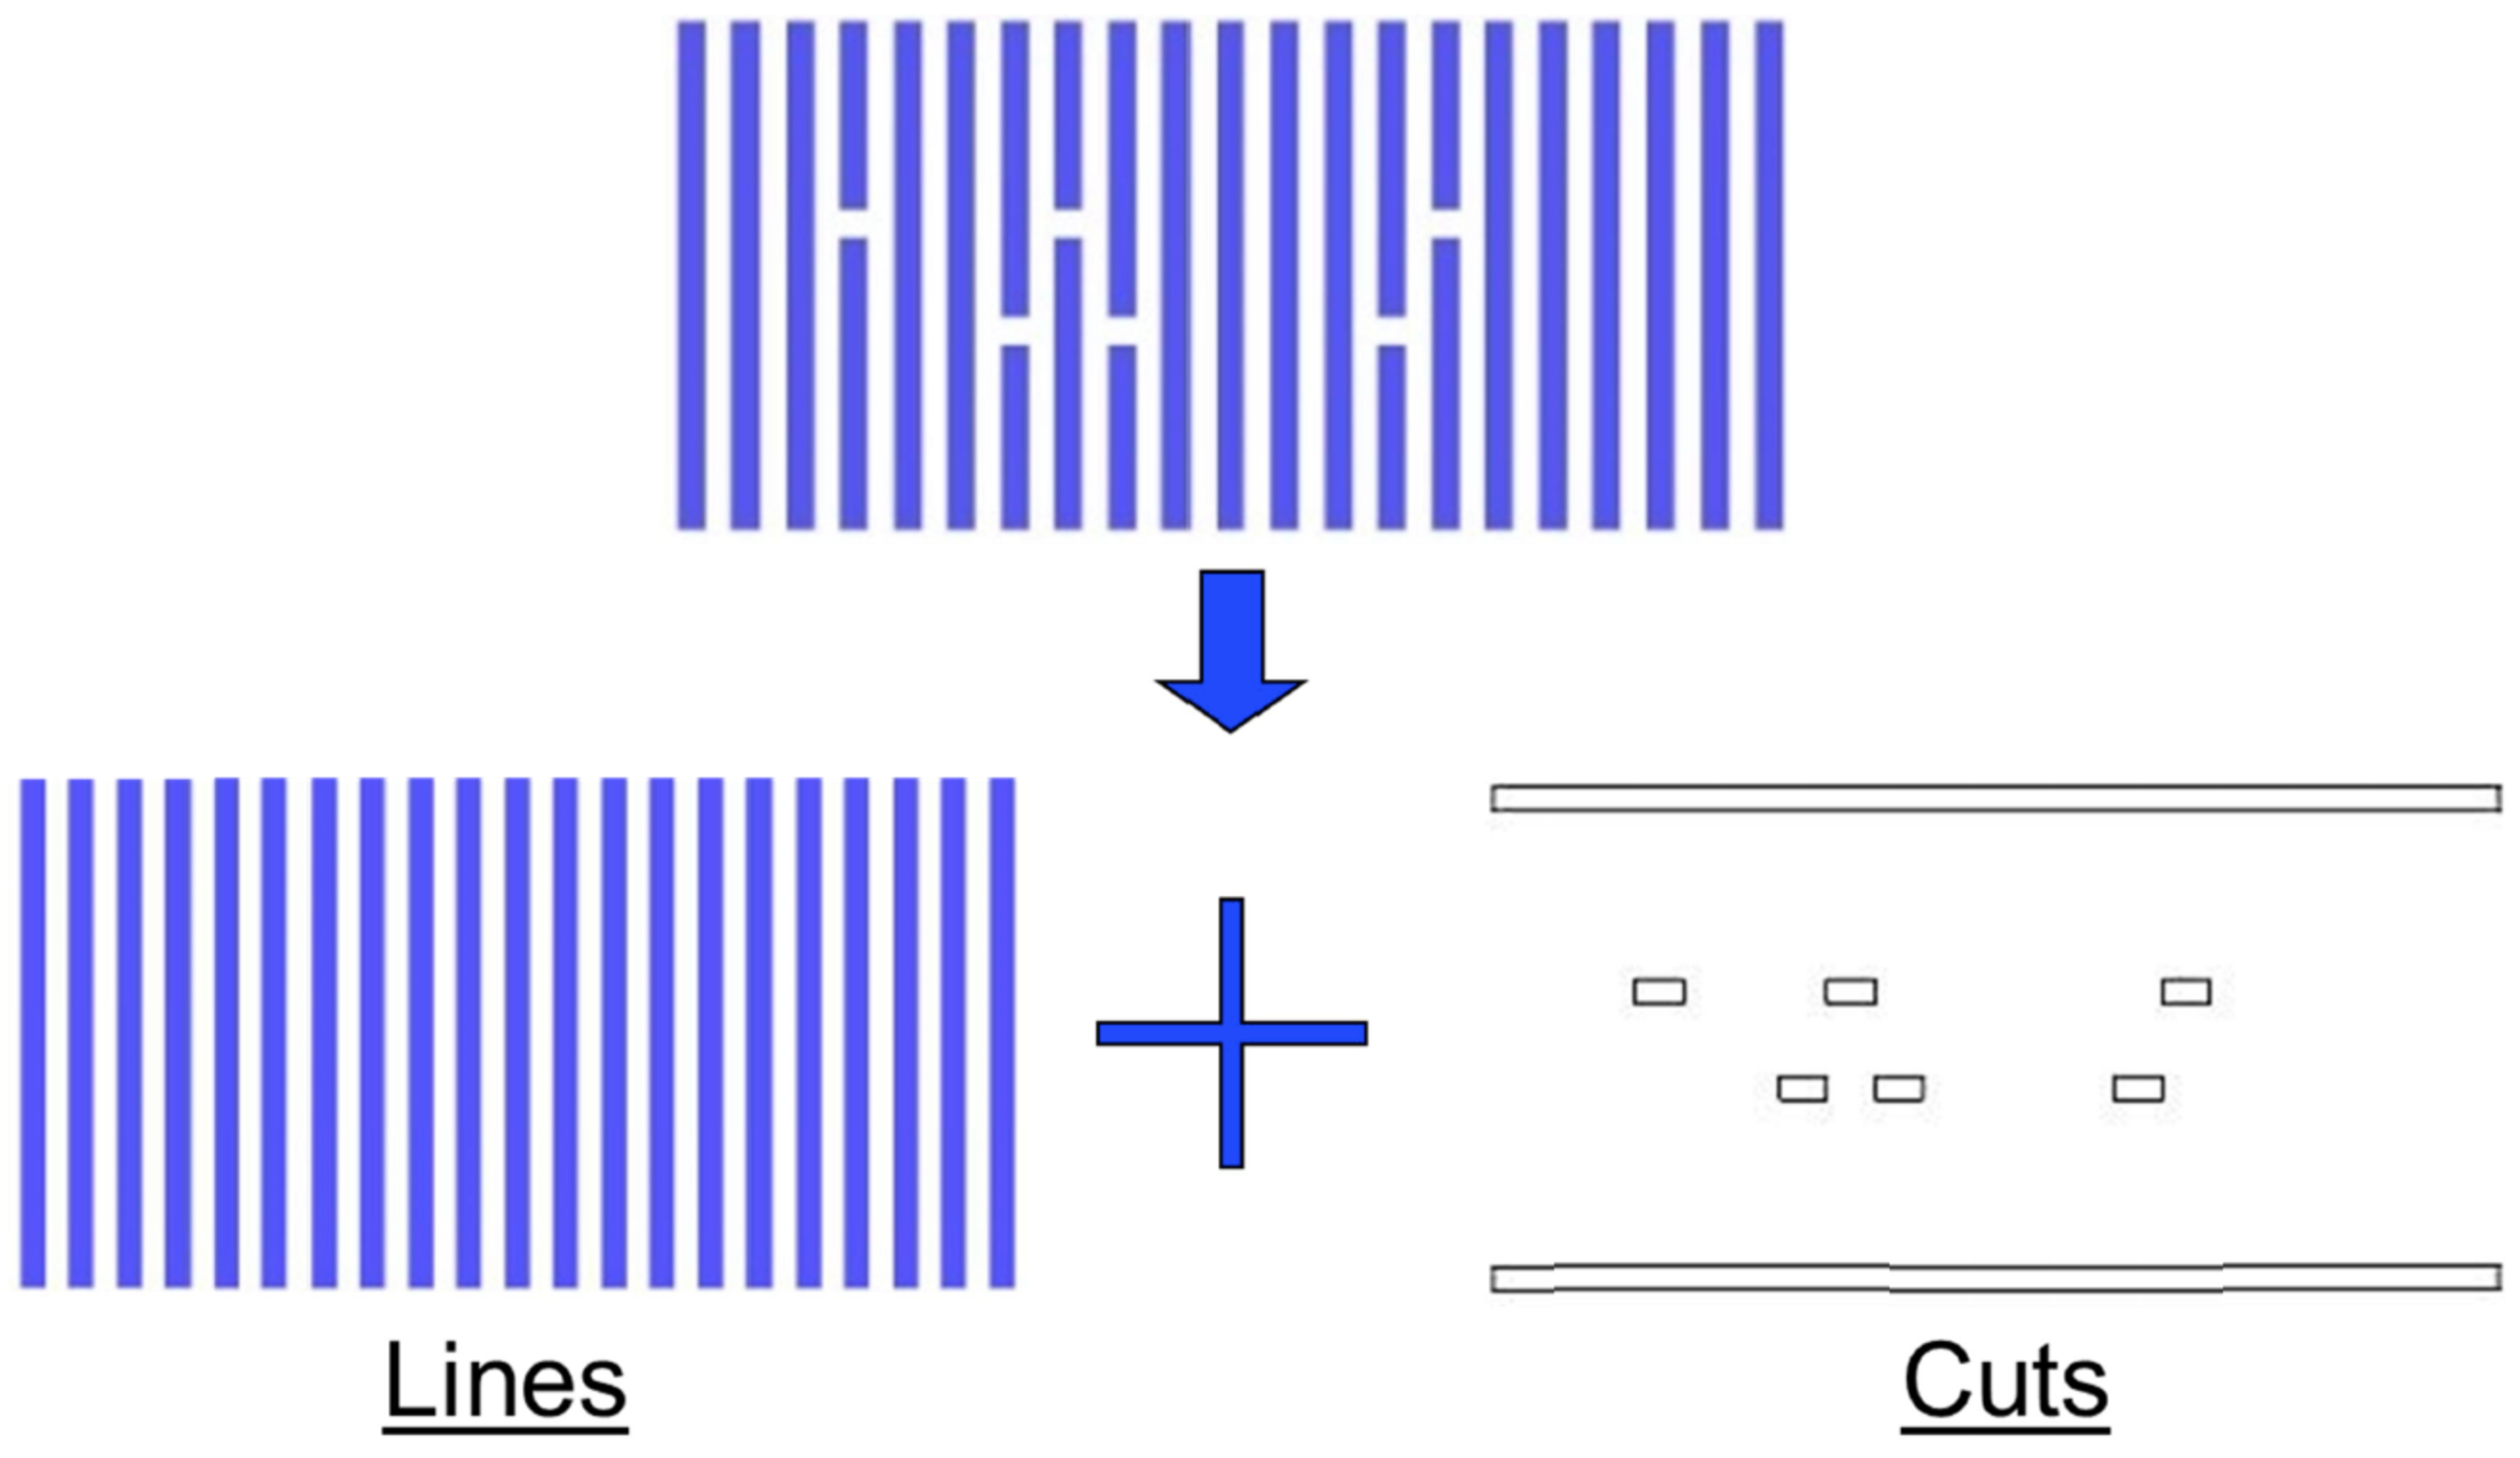
\includegraphics[width=.44\textwidth]{SPIE13_1D_style}
%     \caption{Regular design can be decomposed into lines and cuts \cite{CELL_SPIE2013_Smayling}.}
%     \label{fig:spie13_1d_style}
% \end{figure}

\bibliographystyle{plain}
\begin{thebibliography}{10}

\bibitem{Gartner_IoT_2020}
Gartner Research Inc., ``The Internet of Things'', Press Release, November 2015, \url{http://www.gartner.com/newsroom/id/3165317} .

\bibitem{SwarmAtEdgeOfCloud}
Edward A. Lee, Jan Rabaey, David Blaauw, Kevin Fu, Carlos Guestrin, Bjorn Hartmann, Roozbeh Jafari, Doug Jones, John Kubiatowicz, Vijay Kumar, Rahul Mangharam, Richard Murray, George Pappas, Kris Pister, Anthony Rowe, Alberto Sangiovanni-Vincentelli, Sanjit A. Seshia, Tajana Simunic Rosing, Ben Taskar, John Wawrzynek, David Wessel, ``The Swarm at the Edge of the Cloud'', Design \& Test, IEEE, Volume 31, 2014.

\bibitem{NITrendWatch2016}
National Instruments, ``NI Trend Watch 2016'', \url{http://www.ni.com/pdf/company/en/Trend_Watch_2016_Full.pdf}, accessed Jan 12th, 2016.

\bibitem{MCMHandbook}
A. Davies. ``Handbook of Condition Monitoring: Techniques and Methodology'',  Springer Science \& Business Media, 1997.
%kinda old?

\bibitem{ResarchandMarkets15}
Research and Markets, ``Machine Condition Monitoring Market by Monitoring Type, Components, Monitoring Process``, Applications, and Geography - Global Trend \& Forecast to 2020,
November 2015.

%\bibitem{MCM_NI}
%National Instruments, ``Machine Condition Monitoring Technical Library,'' %\emph{\url{http://www.ni.com/white-paper/6511/en}}, accessed Jan 12th, 2016.

\bibitem{Randall_VibrationbasedCM}
Robert Bond Randall, 
``Vibration-based Condition Monitoring: Industrial, Aerospace and Automotive Applications'', 
John Wiley \& Sons, 2011.
%Cited by 275

\bibitem{InsightCMBrochure15}
National Instruments, ``NI InsightCM\textsuperscript{TM} Enterprise for Condition Monitoring,'' \url{ftp://ftp.ni.com/pub/branches/asean/2015_05_29_insightcm.pdf}, accessed Jan 12th, 2016.

\bibitem{ni_crio}
National Instruments, ``NI Compact RIO'', \url{www.ni.com/compactrio} .

\bibitem{MCM_UC_NI}
National Instruments, ``Featured Machine Condition Monitoring Case Studies,'' \url{http://www.ni.com/white-paper/12398/en}, accessed Jan 12th, 2016.

\bibitem{dukewebsite}
Duke Energy, \url{https://www.duke-energy.com/}, accessed Jan 20th, 2016.

\bibitem{duke}
National Instruments, ``NIWeek 2014 NI InsightCM\textsuperscript{TM} Enterprise Announcement
,'' \url{http://www.ni.com/white-paper/52392/en/}, accessed Jan 20th, 2016.

% \bibitem{LITH_TCAD2013_Pan}
% D.~Z. Pan, B.~Yu, and J.-R. Gao, ``Design for manufacturing with emerging
%   nanolithography,'' \emph{IEEE Transactions on Computer-Aided Design of
%   Integrated Circuits and Systems (TCAD)}, vol.~32, no.~10, pp. 1453--1472,
%   2013.

% \bibitem{CELL_SPIE2013_Smayling}
% M.~C. Smayling, ``{1D} design style implications for mask making and {CEBL},''
%   in \emph{Proceedings of SPIE}, vol. 8880, 2013.

% \bibitem{LITH_SPIE2014_Liebmann}
% L.~Liebmann, V.~Gerousis, P.~Gutwin, M.~Zhang, G.~Han, and B.~Cline,
%   ``Demonstrating production quality multiple exposure patterning aware routing
%   for the 10nm node,'' in \emph{Proceedings of SPIE}, vol. 9053, 2014.



\end{thebibliography}

